\documentclass{beamer}
\usepackage{times}
\usepackage{tikz}
\usepackage{beamerthemesplit}


\title{A Tutorial of White-Box Cryptography \\ Chapter 1 Overview}
\author{Zheng Gong\inst{1,2}\\ \url{cis.gong@gmail.com}}
\institute{\inst{1}{School of Computer Science, South China Normal University} \\ \inst{2}{Mobile Applications And Security Engineering Center of Guangdong Province}}

\date{\today}

\begin{document}

\frame
{
 \titlepage
}

\section[Outline]{}
\frame{\tableofcontents}

\section{Introduction}
\frame
{
  \frametitle{What is cryptology?}

  \textit{``Cryptology is about communication in the presence of \underline{adversaries or potential adversaries}"     \rightline{- R. Rivest}}
  \begin{center}
  \begin{tikzpicture}

        \node[anchor=south west,inner sep=0] (image) at (0,0) {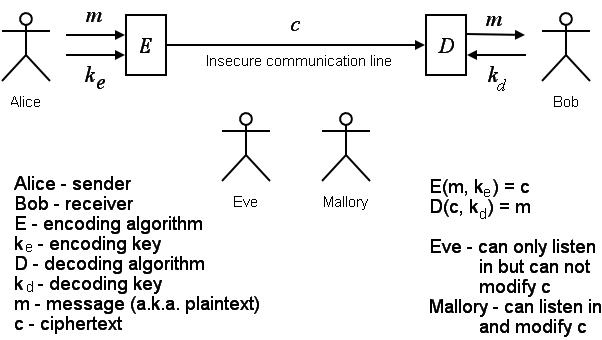
\includegraphics[width=8cm, height=5cm]{./pics/cryptosystem.png}};
        \begin{scope}[x={(image.south east)},y={(image.north west)}]
        %\draw[help lines,xstep=.1,ystep=.1] (0,0) grid (1,1);
        %\foreach \x in {0,1,...,9} { \node [anchor=north] at (\x/10,0) {0.\x}; }
        %\foreach \y in {0,1,...,9} { \node [anchor=east] at (0,\y/10) {0.\y}; }
        \draw[black, thin, rounded corners] (-0.1,0.0) rectangle (1.1,1.0);

    \end{scope}

  \end{tikzpicture}
        \end{center}
}

\frame
{
  \frametitle{What is cryptography?}

\begin{tikzpicture}
    \node[anchor=south west,inner sep=0] (image) at (0,0) { 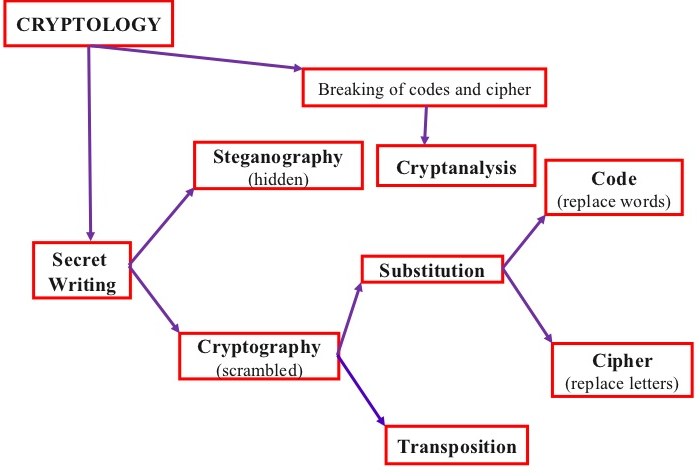
\includegraphics[width=10cm, height=6cm]{./pics/cryptography.png}};

    \begin{scope}[x={(image.south east)},y={(image.north west)}]
        %\draw[help lines,xstep=.1,ystep=.1] (0,0) grid (1,1);
        %\foreach \x in {0,1,...,9} { \node [anchor=north] at (\x/10,0) {0.\x}; }
        %\foreach \y in {0,1,...,9} { \node [anchor=east] at (0,\y/10) {0.\y}; }
        \draw[green, ultra thick, rounded corners] (0.24,0.18) rectangle (0.50,0.32);
    \end{scope}
\end{tikzpicture}

}

\frame
{
 \frametitle{What we need for cryptography?}

 \begin{itemize}
 \setlength{\itemsep}{12pt}
 %\setlength{\parsep}{0pt}
 %\setlength{\parskip}{0pt}
 %\textcolor{red/blue/green/black/white/cyan/magenta/yellow}{text}
 \item \textcolor{red}{\underline{C}onfidentiality}: not just mean en/decryption, it imposes allow authorized people access privileged data
 \item \textcolor{magenta}{\underline{I}ntegrity}: not just mean signature, it includes how to prove the originality and the tractability of the data
 \item \textcolor{blue}{\underline{A}pplicability}: The cryptosystems must be practical
 \end{itemize}
}

\frame
{
\frametitle{Kerckhoffs principle}
\begin{columns}[c]
\column{.65\textwidth}
\begin{itemize}
\setlength{\itemsep}{12pt}
\item Do not rely on keeping an algorithm secret
\item Publish an algorithm but keep the key secretly
\item \textcolor{red}{Have some mathematical foundation for the belief that it will be hard to extract the key}
\end{itemize}

\column{.35\textwidth}
\begin{figure}[htbp]
\centering
  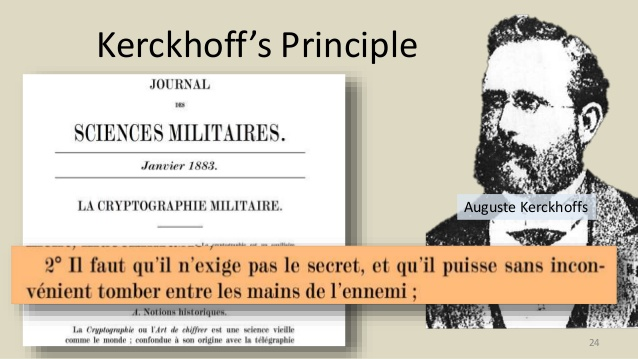
\includegraphics[width=4cm]{./pics/Kerckhoff.jpg}
\end{figure}

\end{columns}
}

\frame
{
\frametitle{Different key types in cryptosystems}
\begin{center}
\begin{tikzpicture}
    \node[anchor=south west,inner sep=0] (image) at (0,0) { 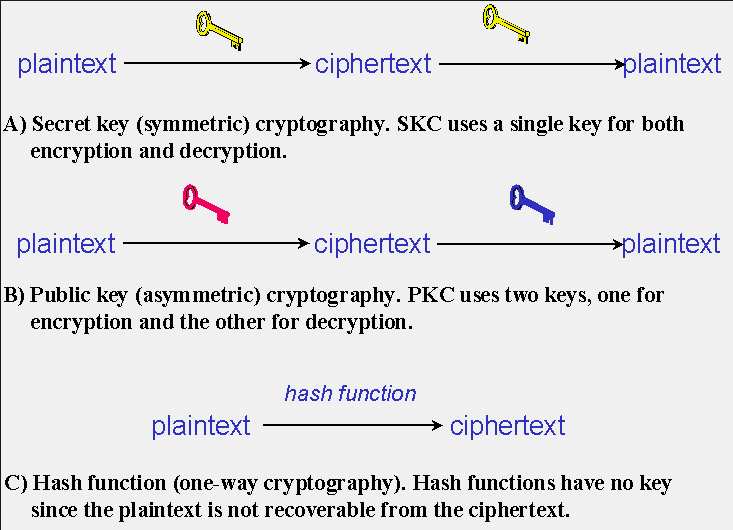
\includegraphics[width=8.5cm, height=5.5cm]{./pics/crypto_key_types.png}};

    \begin{scope}[x={(image.south east)},y={(image.north west)}]
        %\draw[help lines,xstep=.1,ystep=.1] (0,0) grid (1,1);
        %\foreach \x in {0,1,...,9} { \node [anchor=north] at (\x/10,0) {0.\x}; }
        %\foreach \y in {0,1,...,9} { \node [anchor=east] at (0,\y/10) {0.\y}; }
        \draw[black, thin, rounded corners] (0.0,-0.05) rectangle (1.0,1.05);
        \draw[red,line width=1pt](0.04,0.74)--(0.34,0.74);
        \draw[red,line width=1pt](0.04,0.42)--(0.35,0.42);
        \draw[red,line width=1pt](0.24,0.06)--(0.55,0.06);
        %\draw[line width=2pt,-latex](0,0)--(8,0);
    \end{scope}
\end{tikzpicture}
\end{center}
}

\frame
{
\frametitle{Threat model of secret key (1)}
\begin{itemize}
 \setlength{\itemsep}{12pt}
\item There are three combinations in the mobile application threat model.
\begin{itemize}
\setlength{\itemsep}{12pt}
\item Benign host, Malicious client (APPs?)
\item Malicious host, Malicious client (Cloud service?)
\item Benign host, Benign client (VPN?)
\end{itemize}
\setlength{\itemsep}{12pt}
\item In most of mobile applications, hosts are assumed to be benign whilst client might be malicious or controlled by adversary.
\end{itemize}
}

\frame
{
\frametitle{Threat model of secret key (2)}

\begin{itemize}
 \setlength{\itemsep}{12pt}
 \item Black-box model: the adversary cannot intrude/alternate/observe the inside of the cryptosystem;

 \item Grey-box model: the adversary can \textcolor{red}{partially} intrude/alternate/observe the inside of the cryptosystem;

 \item White-box model: the adversary can \textcolor{red}{fully} intrude/alternate/observe the inside of the cryptosystem;
\end{itemize}
}

\frame
{
\frametitle{Applications of black/grey-model-secure products}
\begin{columns}[c]
\column{.6\textwidth}
\begin{itemize}
\item A typical example is the maturing of USB keys
\item The various manufactories and vendors provide different solutions to make RSA/ECC onboard (which also deliberately design to resist grey-box attackers).
\item Eventually it works like a secure black box (and still evolving)
\end{itemize}
\column{.4\textwidth}
\begin{figure}[htbp]
\centering
  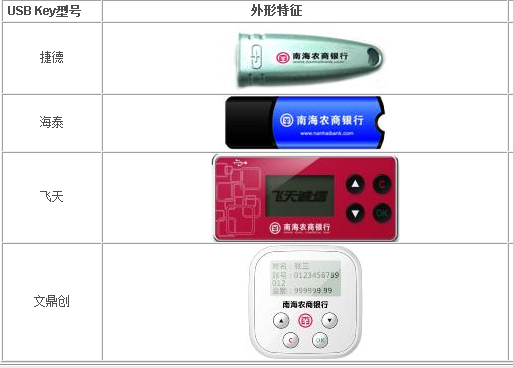
\includegraphics[width=4.8cm]{./pics/usbkey.png}
\end{figure}

\end{columns}

}

\frame
{
\frametitle{Software protection techniques}
\begin{itemize}
\item \textcolor[rgb]{1.00, 0.00, 0.00}{Reverse engineering attacks} - \textcolor[rgb]{0.00,1.00,0.00}{Code obfuscation}

\item \textcolor[rgb]{1.00, 0.00, 0.00}{Modification attacks} - \textcolor[rgb]{0.00,1.00,0.00}{Tamper resistance}

\item \textcolor[rgb]{1.00, 0.00, 0.00}{Program-based attacks} - \textcolor[rgb]{0.00,1.00,0.00}{Software diversity}

\item \textcolor[rgb]{1.00, 0.00, 0.00}{BORE (Break Once Run Everywhere) attacks} - \textcolor[rgb]{0.00,1.00,0.00}{Online/Offline registration verification}
\end{itemize}

In direct usage, \textcolor[rgb]{1.00, 0.00, 0.00}{white-box cryptography} can only solve the key recovery attacks and diversity problems. But it might be a building
block for supporting code obfuscation, tamper resistance, software diversity and registration verification protection.
}

\frame
{
\frametitle{Hardware-aided software key security}
In practice, many kinds of hardware are used to protect software \textcolor[rgb]{1.00, 0.00, 0.00}{key security}.
\begin{columns}[c]
\column{.6\textwidth}
\begin{itemize}
\setlength{\itemsep}{12pt}
\item Environment validation: TPMs
\item Authenticity: USB keys, TPMs
\item Functionality: SE, Crypto ICs, Software USB doggles
\end{itemize}
\column{.4\textwidth}
\begin{figure}[htbp]
\centering
  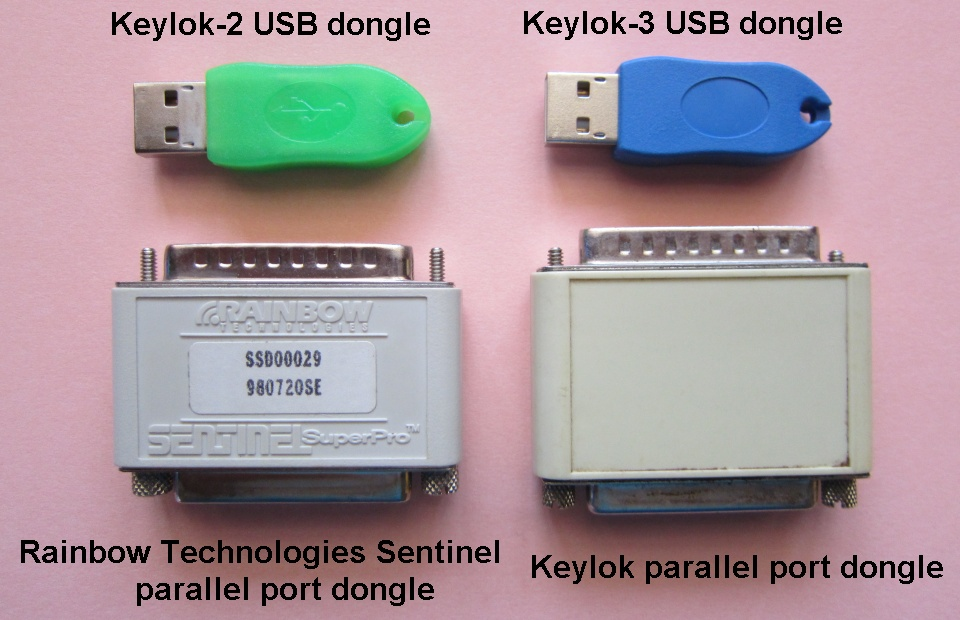
\includegraphics[width=4.8cm]{./pics/dongles.jpg}
\end{figure}

\end{columns}
}

\frame
{
\frametitle{A typical white-box block cipher in a nutshell}
\begin{figure}[htbp]
\centering
  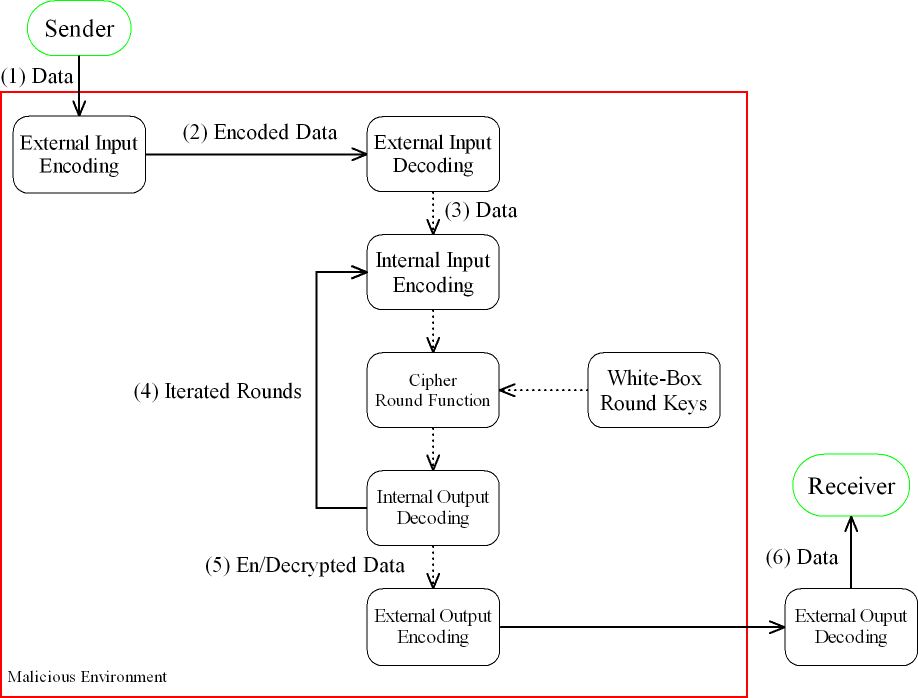
\includegraphics[width=4.8cm]{./pics/WBCrypto_Functional_Model.jpg}
\end{figure}

}


\frame
{
\frametitle{Why we need white-box crypto?}
\begin{itemize}
\setlength{\itemsep}{12pt}
\item Although hardware-protected black/grey-box solutions are matured in the last decade, software solutions are still useful in many areas.

\item To the best of my knowledge, the white-box crypto (which includes symmetric/asymmetric-key cryptosystems) is pivotal for the following practical issues.
\begin{itemize}
\setlength{\itemsep}{12pt}
\item Hardware protection is costly (\textcolor{red}{price})
\item Hardware solution is incompatible (\textcolor{red}{interoperability})
\item Extreme system security protection (\textcolor{red}{key obfuscation})
\item Algorithm implementation flexibility and complexity (\textcolor{red}{Complex functionality requirements})
\end{itemize}
\end{itemize}

}

\frame
{
\frametitle{``counter-examples" on the hardware interoperability}

\begin{figure}
\centering
\begin{minipage}[b]{0.3\textwidth}
\centering
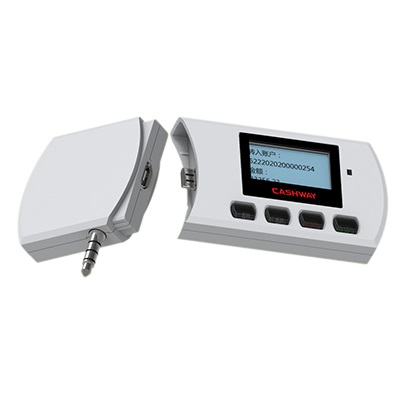
\includegraphics[width=3cm]{./pics/mickey.jpg}
%\parbox{.45\linewidth}{\centering\small a.aa}
\end{minipage}%
\hspace{0.04\textwidth}%
\begin{minipage}[b]{0.3\textwidth}
\centering
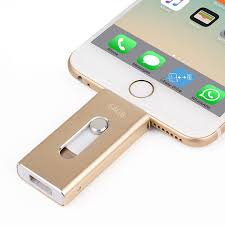
\includegraphics[width=3cm]{./pics/iphonekey.jpeg}
%\parbox{.45\linewidth}{\centering\small b.bb}
\end{minipage}\\[20pt]
\begin{minipage}[b]{0.3\textwidth}
\centering
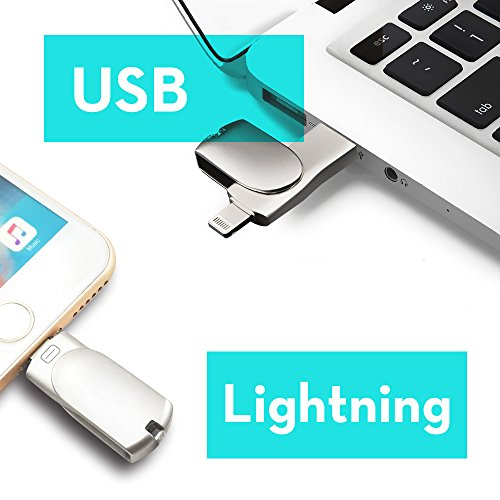
\includegraphics[width=2.7cm]{./pics/usb-lightning.jpg}
%\parbox{.45\linewidth}{\centering\small c.cc}
\end{minipage}
\begin{minipage}[b]{0.3\textwidth}
\centering
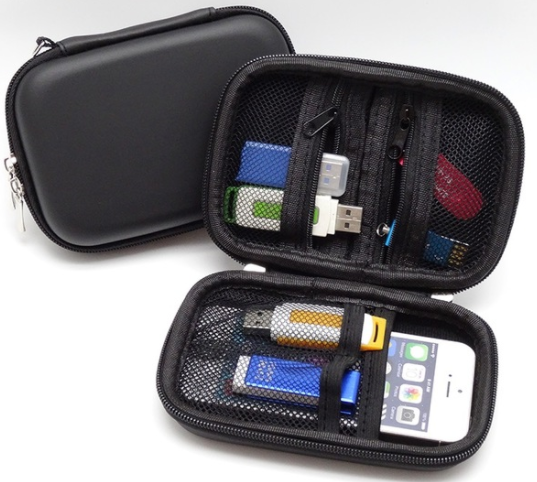
\includegraphics[width=3cm]{./pics/keyproblem.png}
%\parbox{.45\linewidth}{\centering\small c.cc}
\end{minipage}
\end{figure}
}

\frame
{
\frametitle{Threat in software solutions}
Although software solutions enjoy the interoperability and flexibility, the security problems rise.
\begin{itemize}
\setlength{\itemsep}{12pt}
\item emulation
\item run step-by-step in a debugger
\item disassemble/decompile
\end{itemize}

One usually refers to the above attacks as a \textcolor{red}{\textit{white-box}} adversary.
}

\section{Preliminaries of white-box cryptography}
\frame
{
\frametitle{Informal definitions of white-box crypto (1)}
Informally I have the following concerns about white-box crypto:
\begin{itemize}
\setlength{\itemsep}{12pt}
\item From the view of crypto key security, it implies
\begin{itemize}
\setlength{\itemsep}{12pt}
\item secret key protection: adversary cannot extract secret key from software (no matter whether running or not)

\item key distribution mechanism: only designated user/server can generate the white-box version secret key (quite close to public-key crypto, but not exactly the same)

\end{itemize}
\end{itemize}
}

\frame
{
\frametitle{Informal definitions of white-box crypto (2)}
\begin{itemize}
\setlength{\itemsep}{12pt}
\item From the view of software developer, it implies
\begin{itemize}
\setlength{\itemsep}{12pt}
\item cryptographic obfuscation: the algorithm is public, but only the secret key is obfuscated

\item code/space/time hardness: the time/memory/space complexities will increased (heavily)

\item Function abstraction: After white-box implementation, a function's inner functionality is no longer publicly verifiable
\end{itemize}
\end{itemize}

}

\frame
{
\frametitle{Differences between software obfuscation and white-box crypto}
Software obfuscation and white-box crypto can operate together to achieve concrete security, while they have different purposes:
\begin{itemize}
\setlength{\itemsep}{12pt}
\item Software obfuscation does not look for theoretically secure levels of white-box crypto, it should be feasible for practice

\item White-box crypto must be secure either in theory or computational complexity

\item Software obfuscation merely seeks to increase the reverse-engineering costs in a sufficiently discouraging manner for adversary
\end{itemize}

}

\frame
{
\frametitle{White-box crypto working range}
\begin{itemize}
\setlength{\itemsep}{12pt}
\item To resist adversary, a software should be secure against:
\begin{itemize}
\setlength{\itemsep}{12pt}
\item Static analysis: from binary code to extract information

\item Dynamic analysis: from memory to extract information

\item Code lift: change the execution order/function, which breaks the integrity of software
\end{itemize}

\item For white-box crypto, we mainly focus on
\begin{itemize}
\setlength{\itemsep}{12pt}
\item functionality is executed as designed

\item key is not leaked
\end{itemize}

\end{itemize}

}



\frame
{
\frametitle{Basic security definitions for white-box crypto (1)}
\begin{itemize}
\item In SAC 2002, the security notions have  been informally described for white-box cryptography by Chow \textit{et al.}. First the key recovery problem is informally defined by \textcolor{red}{the weak white-box security}
\end{itemize}


\begin{center}
\begin{tikzpicture}
    \node[anchor=south west,inner sep=0] (image) at (0,0) { 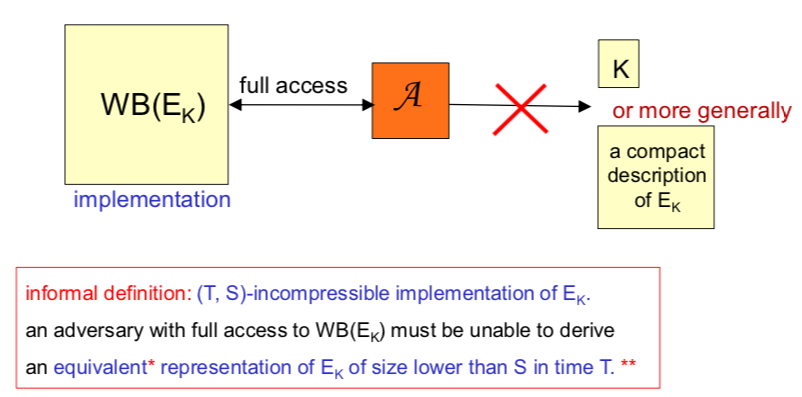
\includegraphics[width=8cm, height=4cm]{./pics/weak_white_box_security.png}};

    \begin{scope}[x={(image.south east)},y={(image.north west)}]
        %\draw[help lines,xstep=.1,ystep=.1] (0,0) grid (1,1);
        %\foreach \x in {0,1,...,9} { \node [anchor=north] at (\x/10,0) {0.\x}; }
        %\foreach \y in {0,1,...,9} { \node [anchor=east] at (0,\y/10) {0.\y}; }
        \draw[red, thin, rounded corners] (0.85,0.7) circle (1.2cm);
    \end{scope}
\end{tikzpicture}
\end{center}
}

\frame
{
\frametitle{Basic security definitions for white-box crypto(2)}
\begin{itemize}
\item For more general security, \textcolor{red}{the strong white-box security} has been defined by Chow et al.
\end{itemize}

\begin{center}
\begin{tikzpicture}
    \node[anchor=south west,inner sep=0] (image) at (0,0) { 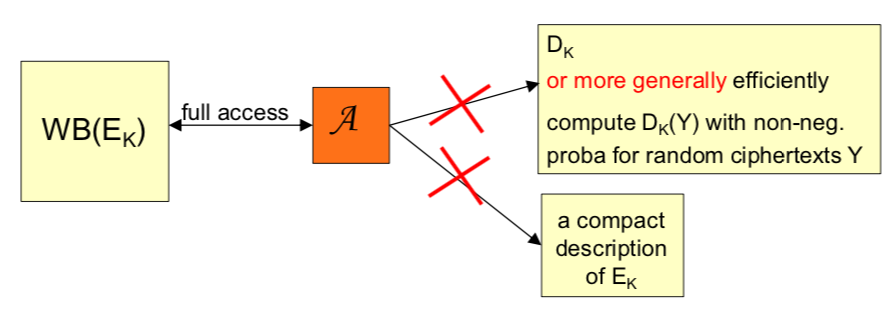
\includegraphics[width=10cm, height=4cm]{./pics/strong_white_box_security.png}};

    %\begin{scope}[x={(image.south east)},y={(image.north west)}]
        %\draw[help lines,xstep=.1,ystep=.1] (0,0) grid (1,1);
        %\foreach \x in {0,1,...,9} { \node [anchor=north] at (\x/10,0) {0.\x}; }
        %\foreach \y in {0,1,...,9} { \node [anchor=east] at (0,\y/10) {0.\y}; }
        %\draw[green, ultra thick, rounded corners] (0.24,0.18) rectangle (0.50,0.32);
    %\end{scope}
\end{tikzpicture}
\end{center}
}

\section{The State-of-the-art of WBC}

\section{Conclusion}

\frame
{
\frametitle{}

\begin{itemize}
\setlength{\itemsep}{12pt}
\item Software security is significant for protecting applications in practice

\item Software obfuscation and white-box cryptography are different fruits on same tree

\item Applications have various requirements on white-box crypto

\end{itemize}

}

\frame
{
\begin{center}
\textbf{Thanks for your attentions!}

\end{center}

\begin{center}
\begin{tikzpicture}
    \node[anchor=south west,inner sep=0] (image) at (0,0) { 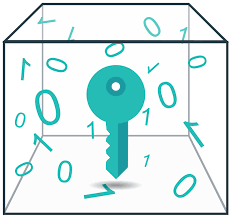
\includegraphics[width=4cm, height=4cm]{./pics/WBC_BG.png}};

    %\begin{scope}[x={(image.south east)},y={(image.north west)}]
        %\draw[help lines,xstep=.1,ystep=.1] (0,0) grid (1,1);
        %\foreach \x in {0,1,...,9} { \node [anchor=north] at (\x/10,0) {0.\x}; }
        %\foreach \y in {0,1,...,9} { \node [anchor=east] at (0,\y/10) {0.\y}; }
        %\draw[green, ultra thick, rounded corners] (0.24,0.18) rectangle (0.50,0.32);
    %\end{scope}
\end{tikzpicture}

\end{center}
}

\end{document}
